\chapter{Les vecteurs}

Dans l'introduction, nous avons parlé de mouvement, de position et nous avons
mentionné le concept de déplacement.  Le \textbf{déplacement} est simplement un
changement de position.  Si je me déplace de trois mètres, je peux me trouver à
une infinité de positions différentes parce que je n'ai pas précisé dans quelle
direction je me déplace.  Pour qu'un déplacement soit clairement définie, il
faut donner à la fois une longueur et une direction.  Les quantités qui sont
définies de la sorte sont appelées des \textbf{vecteurs}.
\marginnote{Le mot \textit{vecteur} vient du latin \textit{veho} qui veut dire
transporter.}

\begin{defn}[vecteur]
  Un \textbf{vecteur} est une quantité qui est définie par une \textbf{norme}
  (ou \textbf{longueur} ou \textbf{module}) et une \textbf{direction}.
\end{defn}

Un vecteur a une \textbf{origine} et une \textbf{extrémité}.  Tous les vecteurs
sont représentés par un symbole surmonté d'une flèche, par exemple $\vec{v}$.

\begin{center}
\begin{tikzpicture}[scale=1]
  \draw[->] (0, 0) -- node[above] {$\vec{v}$} (3, 2); 
\end{tikzpicture}
\end{center}

\textbf{Il est extrêmement important de ne pas oublier la flèche au-dessus des
vecteurs.}

La norme du vecteur $\vec{a}$ est notée $\norm{\vec{a}}$ ou simplement $a$ sans la
flèche.  Ainsi, les quantités $\vec{a}$ et $a$ sont complètement différentes.

Voici quelques exemples de vecteurs que nous utiliserons en physique : la
position, le déplacement, la vitesse, l'accélération, la force, le champ
électrique, etc.

Un \textbf{scalaire} est une quantité qui est décrite entièrement par un seul
nombre.  Les quantités suivantes sont des scalaires : le temps, la température,
la distance parcourue, l'énergie, le travail, la norme d'un vecteur, etc.


\section{Addition géométrique de vecteurs}

Schklaktonek lance une rondelle de hockey du point $A$ au point $B$ où Pianotta
la reçoit et l'envoie vers le filet, au point $C$.  Quel est le déplacement
total de la rondelle?

\begin{marginfigure}
  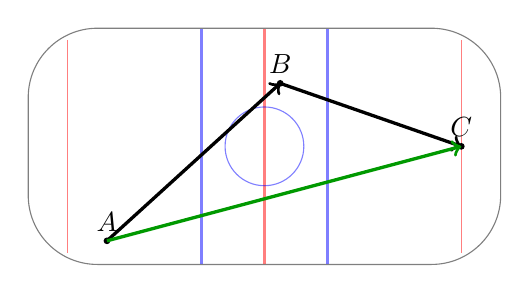
\begin{tikzpicture}
    \begin{scope}[opacity=0.5]
      \draw[rounded corners=25] (0, 0) rectangle (6, 3);
      \draw[red] (0.5, 0.15) -- (0.5, 2.85);
      \draw[red] (5.5, 0.15) -- (5.5, 2.85);
      \draw[red, thick] (3, 0.01) -- (3, 2.99);
      \draw[blue, thick] (2.2, 0.01) -- (2.2, 2.99);
      \draw[blue, thick] (3.8, 0.01) -- (3.8, 2.99);
      \draw[blue] (3, 1.5) circle (0.5);
    \end{scope}
    \coordinate (A) at (1, 0.3);
    \coordinate (B) at (3.2, 2.3);
    \coordinate (C) at (5.5, 1.5);
    \coordinate (O) at (1, -1);
    \draw[fill=black] (A) circle (1pt);
    \node[above] at (A) {$A$};
    \draw[fill=black] (B) circle (1pt);
    \node[above] at (B) {$B$};
    \draw[fill=black] (C) circle (1pt);
    \node[above] at (C) {$C$};
    \draw[very thick, ->] (A) -- (B);
    \draw[very thick, ->] (B) -- (C);
    \draw[very thick, ->, green!60!black] (A) --(C);
  \end{tikzpicture}
\end{marginfigure}

En déterminant le déplacement total de la rondelle, nous avons fait une
addition de vecteurs.  Géométriquement, deux vecteurs peuvent être additionnés
en les plaçant tête à queue, puis en traçant le vecteur qui va de l'origine du
premier à l'extrémité du second.

Cette méthode se généralise très bien à la somme de plusieurs vecteurs.  On n'a
qu'à placer tous les vecteurs l'un à la suite de l'autre.  Le vecteur somme est
celui qui va de l'origine du premier à l'extrémité du dernier.

\begin{marginfigure}
  \begin{tikzpicture}[scale=0.6]
    \draw[->] (0, 0) -- node[left] {$\vec{a}$} (1, 4);
    \draw[->, shift={(1, -1)}] (1, 4) -- node[above] {$\vec{b}$} (5, 2);
    \draw[->, shift={(-3, 3)}] (5, 2) -- node[above] {$\vec{c}$} (0, 0);
  \end{tikzpicture}
\end{marginfigure}

Il est possible qu'en plaçant les vecteurs l'un à la suite de l'autre le point
de départ du premier vecteur soit le même que le point d'arrivée du dernier
vecteur.  Lorsque cela se produit, on obtient un vecteur particulier appelé le
\textbf{vecteur nul} et noté $\vec{0}$.

\begin{marginfigure}
  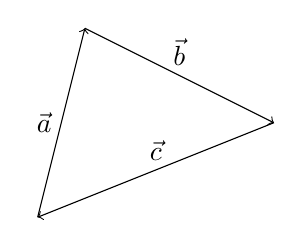
\begin{tikzpicture}[scale=0.6]
    \draw[->] (0, 0) -- node[left] {$\vec{a}$} (1, 4);
    \draw[->] (1, 4) -- node[above] {$\vec{b}$} (5, 2);
    \draw[->] (5, 2) -- node[above] {$\vec{c}$} (0, 0);
  \end{tikzpicture}
\end{marginfigure}

Il est important de distinguer vecteur nul $\vec{0}$ du scalaire zéro $0$.
Les deux quantités sont de types différents.  Un vecteur ne peut jamais être
égal à un scalaire, et il est impossible d'additionner un vecteur à un
scalaire.  Par conséquent, une expression comme $\vec{u} + \vec{0}$ a un sens
alors que $\vec{u} + 0$ n'en a pas.


\section{Multiplication d'un vecteur par un scalaire}

On peut multiplier un vecteur par un scalaire.  Par exemple, $3\vec{v}$ est une
façon d'écrire $\vec{v} + \vec{v} + \vec{v}$.  Ce vecteur a donc la même
orientation que $\vec{v}$, mais sa norme est le triple de celle de $\vec{v}$.

Si on multiplie un vecteur par $-1$, on obtient $-\vec{v}$ qui est un vecteur
dont la norme est la même que celle de $\vec{v}$ mais dont l'orientation est
l'opposée de celle de $\vec{v}$.  Cette définition fait en sorte que si
$\vec{v}$ est un déplacement de $A$ à $B$, alors $-\vec{v}$ est le déplacement
opposé, c'est-à-dire de $B$ à $A$.

À partir de la définition de $-\vec{v}$, on peut définir la soustraction de
vecteurs.  Soustraire deux vecteurs correspond à ajouter au premier vecteur
l'opposé du second:
\[
  \vec{u} - \vec{v} = \vec{u} + (-\vec{v})
\]
La soustraction de vecteurs est souvent utilisée pour calculer un déplacement à
partir des positions initiales et finales.

\begin{marginfigure}
  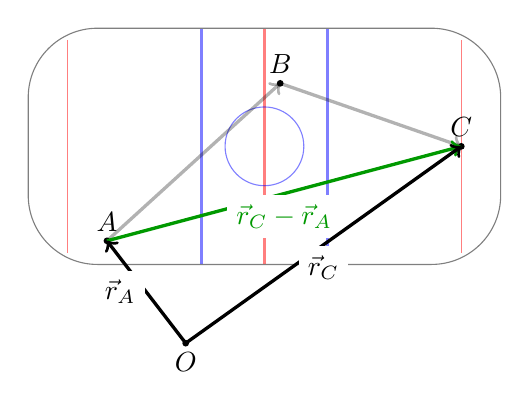
\begin{tikzpicture}
    \begin{scope}[opacity=0.5]
      \draw[rounded corners=25] (0, 0) rectangle (6, 3);
      \draw[red] (0.5, 0.15) -- (0.5, 2.85);
      \draw[red] (5.5, 0.15) -- (5.5, 2.85);
      \draw[red, thick] (3, 0.01) -- (3, 2.99);
      \draw[blue, thick] (2.2, 0.01) -- (2.2, 2.99);
      \draw[blue, thick] (3.8, 0.01) -- (3.8, 2.99);
      \draw[blue] (3, 1.5) circle (0.5);
    \end{scope}
    \coordinate (A) at (1, 0.3);
    \coordinate (B) at (3.2, 2.3);
    \coordinate (C) at (5.5, 1.5);
    \coordinate (O) at (2, -1);
    \draw[fill=black] (O) circle (1pt);
    \node[below] at (O) {$O$};
    \draw[fill=black] (A) circle (1pt);
    \node[above] at (A) {$A$};
    \draw[fill=black] (B) circle (1pt);
    \node[above] at (B) {$B$};
    \draw[fill=black] (C) circle (1pt);
    \node[above] at (C) {$C$};
    \draw[very thick, ->, opacity=0.3] (A) -- (B);
    \draw[very thick, ->, opacity=0.3] (B) -- (C);
    \draw[very thick, ->, green!60!black] (A)
         -- node[below, fill=white] {$\vec{r}_C - \vec{r}_A$} (C);
    \draw[very thick, ->] (O) -- node[left, fill=white] {$\vec{r}_A$} (A);
    \draw[very thick, ->] (O) -- node[below, fill=white] {$\vec{r}_C$} (C);
  \end{tikzpicture}
\end{marginfigure}

Il existe deux méthodes équivalentes pour calculer une différence de vecteurs.
La première consiste à trouver l'opposé du vecteur qu'on soustrait puis à
l'additionner à celui duquel on soustrait.  La seconde consiste à placer les
deux vecteurs de telle sorte qu'ils aient la même origine.  Le vecteur
différence est alors celui qui va de l'extrémité du vecteur qu'on soustrait à
l'extrémité de celui duquel on soustrait.


\section{Addition algébrique de vecteurs}

L'approche géométrique pour additionner des vecteurs est utile, mais lorsqu'on
veut obtenir un résultat quantitatif, il est préférable d'utiliser une méthode
algébrique.  Dans un système de coordonnées cartésiennes en deux (resp. trois)
dimensions, on utilise deux (resp. trois) vecteurs particuliers pour
\textbf{décomposer} tous les autres vecteurs.

Ces vecteurs particuliers sont les vecteurs unitaires $\xhat$, $\yhat$ et
$\zhat$.  Un \textbf{vecteur unitaire} est un vecteur dont la longueur est une
unité, $1$.  Les vecteurs $\xhat$, $\yhat$ et $\zhat$ sont dirigés vers la
direction positive des axes $x$, $y$ et $z$ respectivement.

\begin{marginfigure}
  \begin{tikzpicture}[scale=4]
    \draw[->] (0, 0, 0) -- (1, 0, 0) node[right] {$y$};
    \draw[->] (0, 0, 0) -- (0, 1, 0) node[left] {$z$};
    \draw[->] (0, 0, 0) -- (0, 0, 1) node[below] {$x$};
    \draw[->, ultra thick] (0, 0, 0) -- (0.6, 0, 0) node[above] {$\yhat$};
    \draw[->, ultra thick] (0, 0, 0) -- (0, 0.6 0) node[right] {$\zhat$};
    \draw[->, ultra thick] (0, 0, 0) -- (0, 0, 0.6) node[anchor=south east] {$\xhat$};
    \draw (0.6, 0, 0) -- (0.6, -0.05, 0) node[below] {$1$};
    \draw (0, 0.6, 0) -- (-0.05, 0.6, 0) node[left] {$1$};
    \draw (0, 0, 0.6) -- (0.05, 0, 0.6) node[below] {$1$};
  \end{tikzpicture}
\end{marginfigure}

N'importe quel vecteur peut s'écrire comme une somme de multiples des vecteurs
unitaires $\xhat$, $\yhat$ et $\zhat$:
\[
  \vec{v} = v_x \xhat + v_y \yhat + v_z \zhat
\]
où $v_x$, $v_y$ et $v_z$ sont les \textbf{composantes} du vecteur $\vec{v}$
le long des axes $x$, $y$ et $z$.  Les composantes d'un vecteur sont des
scalaires qui peuvent être positifs ou négatifs.

Si on connaît les composantes de deux vecteurs on peut les additionner
facilement.  Par exemple, si $\vu = u_x \xhat + u_y\yhat + u_z\zhat$ et
$\vv = v_x \xhat + v_y\yhat + v_z\zhat$, alors on peut calculer la somme
directement:
\begin{align*}
  \vu + \vv &= (u_x \xhat + u_y\yhat + u_z\zhat)
             + (v_x \xhat + v_y\yhat + v_z\zhat) \\
            &= (u_x + v_x) \xhat + (u_y + v_y) \yhat + (u_z + v_z) \zhat
\end{align*}
Autrement dit, l'addition se fait composante par composante.

\begin{marginfigure}
  \begin{tikzpicture}[scale=1]
    \draw[->] (-1, 0) -- (4, 0) node[below] {$x$};
    \draw[->] (0, -1) -- (0, 4) node[left] {$y$};
    \draw[very thick, ->] (0, 0) -- node[above] {$\vec{v}$} (3, 2);
    \draw[very thick, ->, blue] (0, 0) -- (3, 0);
    \draw[very thick, ->, red] (3, 0) -- (3, 2);
  \end{tikzpicture}
\end{marginfigure}
Pourquoi tout cela a-t-il un sens? Pour le voir, il est plus simple de se
concentrer sur le cas à deux dimensions.  Considérons un vecteur $\vv$.  Ce
vecteur peut être vu comme la somme de deux vecteurs perpendiculaires, un le
long de l'axe $x$ et l'autre le long de l'axe $y$.  Le vecteur parallèle à
l'axe $x$ est aussi parallèle à $\xhat$ et peut donc s'écrire comme un multiple
scalaire de $\xhat$.  On appelle le multiple en question $v_x$.  Un
raisonnement identique permet de définir $v_y$.

Pour déterminer les composantes d'un vecteur $\vv$ dont on connaît la norme
\marginnote{Cela devrait vous rappeler la conversion d'un système de
  coordonnées polaires à un système de coordonnées cartésiennes.}
$v$ et l'orientation $\theta$, on utilise un peu de trigonométrie:
\begin{align*}
  v_x &= v \cos \theta \\
  v_y &= v \sin \theta
\end{align*}


\subsection{Exemple d'addition algébrique I}

\exemple{
  Pour se rendre à l'endroit où il doit sauver des naufragés, un pilote
  d'hélicoptère décolle de l'aéroport et parcourt \SI{20}{\kilo\meter} vers le
  nord-ouest.  Il bifurque ensuite de \SI{60}{\degree} vers sa droite et
  parcourt un autre \SI{45}{\kilo\meter}.

  En utilisant la décomposition des vecteurs en fonction des vecteurs
  unitaires, déterminer le déplacement total effectué par le pilote.

  \begin{tikzpicture}[scale=1]
    \draw[->] (-2, 0) -- (1, 0) node[right] {$x$};
    \draw[->] (0, -1) -- (0, 6) node[left] {$y$};
    \coordinate (A) at (0, 0);
    \coordinate (B) at ($(0, 0) + (135:2)$);
    \coordinate (C) at ($(B) + (75:4.5)$);
    \draw[dashed] (A) -- ($1.4*(B)$);
    \draw[->, very thick] (A) -- node[below] {$\vu$} (B);
    \draw (0, 0.6) arc (90:135: 0.6);
    \node at (-0.3, 0.8) {\SI{45}{\degree}};
    \draw ($(B) + 0.1*(75:4.5)$) arc (75:135:0.4);
    \node at (-1.6, 2.2) {\SI{60}{\degree}};
    \draw[->, very thick] (B) -- node[left] {$\vv$} (C);
  \end{tikzpicture}

  Simplement avec la figure, on sait que la composante en $x$ du déplacement
  sera négative alors que la composante en $y$ sera positive.

  D'abord on décompose les deux vecteurs.  Pour le vecteur $\vu$, on trouve les
  composantes en $x$ et $y$:
  \begin{eqnarray*}
    u_x &= -u \sin \SI{45}{\degree} &= -\SI{20}{\kilo\meter} \sin
      \SI{45}{\degree} = -\SI{14.14213}{\kilo\meter} \\
    u_y &=  u \cos \SI{45}{\degree} &=  \SI{20}{\kilo\meter} \cos
      \SI{45}{\degree} = \SI{14.14213}{\kilo\meter} \\
  \end{eqnarray*}
  Le résultat est donc
  \[
    \vu = (-\num{14.1}\, \xhat + \num{14.1}\, \yhat) \si{\kilo\meter}
  \]
  Pour le vecteur $\vv$, on note que l'angle entre l'axe des $x$ positifs et
  le vecteur est \SI{75}{\degree}.  Par conséquent
  \begin{eqnarray*}
    v_x &= -v \cos \SI{75}{\degree} &= -\SI{45}{\kilo\meter} \cos
      \SI{75}{\degree} = \SI{11.64685}{\kilo\meter} \\
    v_y &=  v \sin \SI{75}{\degree} &=  \SI{45}{\kilo\meter} \sin
      \SI{75}{\degree} = \SI{43.46666}{\kilo\meter} \\
  \end{eqnarray*}
  Le vecteur est donc
  \[
    \vv = (\num{11.6}\, \xhat + \num{43.5}\, \yhat) \si{\kilo\meter}
  \]
  On peut maintenant faire la somme des deux déplacements pour obtenir le
  déplacement total.  Attention!  Pour le calcul de la somme, nous utilisons
  plus de chiffres que trois afin de ne pas être victime d'erreurs d'arrondi.
  \begin{align*}
    \vu + \vv &= (-\num{14.14213}\, \xhat + \num{14.14213}\, \yhat) \si{\kilo\meter}
                +(\num{11.64685}\, \xhat + \num{43.46666}\, \yhat)
                \si{\kilo\meter} \\
              &= (-\num{2.50}\, \xhat + \num{57.6}\, \yhat) \si{\kilo\meter}
  \end{align*}
}


\subsection{Exemple d'addition algébrique II}

\exemple{
  En général, est-ce que $\norm{\vv} + \norm{\vu} = \norm{\vv + \vu}$?

  À partir de la décomposition obtenue à la question sur le pilote
  d'hélicoptère pour chacun des
  deux déplacements, $\vu$ et $\vv$, calculer les quantités suivantes:

  \begin{enumerate}
    \item $\norm{\vv} + \norm{\vu}$
    \item $\norm{\vv + \vu}$
  \end{enumerate}

  À partir des composantes, on peut calculer les normes de chacun des vecteurs.
  \begin{align*}
    \norm{\vu} &= \sqrt{u_x^2 + u_y^2} \\
               &= \sqrt{(\SI{14.14213}{\kilo\meter})^2 + (\SI{14.14213}{\kilo\meter})^2} \\
               &= \SI{20.0}{\kilo\meter}
  \end{align*}
  \begin{align*}
    \norm{\vv} &= \sqrt{v_x^2 + v_y^2} \\
               &= \sqrt{(\SI{11.64685}{\kilo\meter})^2 + (\SI{43.46666}{\kilo\meter})^2} \\
               &= \SI{45.0}{\kilo\meter}
  \end{align*}
  Puis la norme du déplacement total:
  \begin{align*}
    \norm{\vu + \vv} &= \sqrt{(\SI{-2.49528}{\kilo\meter})^2 + (\SI{57.60879}{\kilo\meter})^2} \\
                     &= \SI{57.7}{\kilo\meter}
  \end{align*}
}


\section{Approche algébrique à la multiplication par un scalaire}

Multiplier un vecteur par un scalaire correspond à allonger ou raccourcir le
vecteur, et, si le scalaire est négatif, à renverser son orientation.  Un peu
de réflexion permet de constater que si on allonge le vecteur d'un facteur $k$,
alors chacune des composantes du vecteur allonge d'un facteur $k$.  Autrement
dit, multiplier un vecteur par un scalaire est équivalent à multiplier chacune
des composantes du vecteur par ce même scalaire.

Si $\vv = v_x \xhat + v_y \yhat + v_z \zhat$, alors
\[
  k\vv = kv_x \xhat + kv_y \yhat + kv_z \zhat
\]

\subsection{Exemple d'algèbre vectorielle}

\exemple{
  Deux forces agissent sur un objet:
  \begin{align*}
    \vec{F}_1 &= (3 \xhat - 7 \yhat) N \\
    \vec{F}_2 &= (- \xhat + 5 \yhat) N
  \end{align*}
  Pour une raison quelconque, la deuxième force est soudainement quadruplée et
  son orientation est inversée.  Calculer la force totale qui agit maintenant
  sur l'objet, c'est-à-dire, calculer
  \[
    \vec{F}_1 - 4\vec{F}_2
  \]
}
